\documentclass{article}
\usepackage[utf8]{inputenc}
\usepackage{amsmath}
\usepackage{amsfonts}
\usepackage{graphicx}
\usepackage{multicol}
\usepackage{float}
\usepackage{cite}
\usepackage{url}
\usepackage{listings}
\usepackage{pythonhighlight}
\begin{document}
	\begin{titlepage}
		\begin{center}
			{\huge\textbf{Instituto Politécnico Nacional}}\\
			\vspace{7mm}
			{\huge\textbf{Escuela Superior de Cómputo}}\\			
			\begin{figure}[h]
				\centering
				
\includegraphics[height = 6cm]{logoEscom.png}
			\end{figure}	
			\vspace{1cm}
			{\huge\textbf{Programa 7: Palindromes}}
			\par\vspace{2cm}
			\large\textbf{Autor: Colín Ramiro Joel}
			\par\vspace{1cm}
			{\large\textbf{Materia: Teoría de la Computación}}
			\par\vspace{1cm}
			{\large\textbf{Grupo: 4CM2}}
			\par\vspace{1cm}
			{\large\textbf{Profesor: Juarez Martínez Genaro}}
			\par\vspace{1cm}
			{\large\textbf{Fecha de entrega: {\huge{29 de Diciembre 2021}}}}
			\par\vspace{3cm}
		\end{center}
	\end{titlepage}	
	
	\section*{Introducción}
	En un contexto fuera de las ciencias de la computación, un palindromo es una palabra o frase que se lee igual en un sentido que en otro (derecha a izquierda y viceversa). Habitualmente, las frases palindrómicas se resienten en su significado cuanto más largas son. 
	
	Ya en un contexto compuatcional, no se tiene que tomar necesariamente a los palíndromos como palabras reales en un idioma cualquiera. Se puede tambien pensar en un palíndromo como cualquier secuencia de letras que se lee igual hacia adelante y hacia atrás, como lo puede ser \textbf{xyzyzyx} o un conjunto de números como \textbf{1001001}. Como bien ya se sabe a una secuencia de letras se le conoce como una cadena. Asi entonces se puede considerar que cualquier cadena que contenga una sola letra es, por defecto, un palíndromo. Ahora bien, una cadena puede no contener ninguna letra; a una cadena de cero letras la llamamos una cadena vacía. Esta cadena vacía también es un palíndromo, ya que se "lee" del mismo modo hacia adelante y hacia atrás como bien se definió al inicio de esta sección. Así que ahora consideremos que cualquier cadena que contenga como mínimo una letra es un palíndromo. 
	
	\section*{Instrucciones}
	Realizar un programa que construya palindromes de un lenguaje binario. El lenguaje deberá solicitar únicamente la longitud del palindrome a calcular, de esta manera el programa deberá construir el palindrome de manera aleatoria. La longitud máxima que podría alcanzar un palindrome será de 100,000 caracteres. La salida del programa se irá a un archivo de texto y ahí especificarán qué regla se selecciono y la cadena resultante hasta llegar a la cadena final. El programa deberá ofrecer dos opciones: que el usuario defina la longitud del palindrome o que lo genere todo de manera automática.
	
	
	La gramática libre de contexto que construye palindromes, se define con las siguientes reglas de producción.
	\begin{enumerate}
		\item P $\rightarrow$ e
		\item P $\rightarrow$ 0
		\item P $\rightarrow$ 1
		\item P $\rightarrow$ 0P0
		\item P $\rightarrow$ 1P1	
	\end{enumerate}
	En el reporte debe de estar también el código de la implementación en latex, no en imágenes.
	\section*{Desarrollo}	
	Para la realización de este programa se implementó un menú principal en el cual el usuario seleccionará el modo en el que se introducirá la longitud del palíndromo. Se puede ya sea el modo manual, el automático y además, se puede seleccionar para salir del programa.
	
	Se implementó una función llamada \textbf{palindrome}, la cual dependiendo de la selección del usuario, preguntará cuál es la longitud deseada para el palindromo si se selecciona el modo manual. Por otro lado, si se selcciona el modo automático generará un número aleatorio entre 1 y 100,000 el cual será la longitud del palindromo.
	
	Conforme se va generando el palíndromo, se van aplicando las reglas definidas en el código, estas reglas son las que se especificaron previamente en la sección e Instrucciones. La contucción del palíndromo se específica en el archivo de texto \textbf{"SalidaP7.txt"}
	
	\section*{Capturas del Funcionamiento}
	En esta sección se encuentran las capturas de pantalla del funcionamiento del programa, tanto de la consola, como de los archivos generados.
	Las capturas se ordenaron comforme a la opción selecionada en el programa: 
	\begin{enumerate}
		\item \textbf{Modo Manual}
		\begin{itemize}
			\item 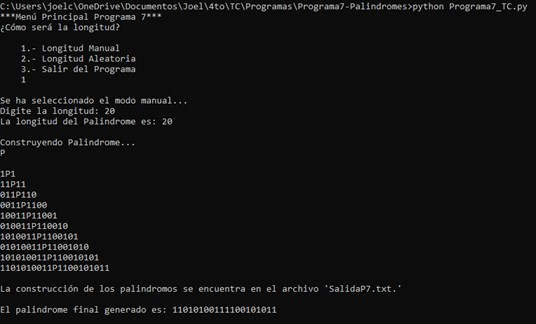
\includegraphics[height = 4cm]{MM1.jpg}
			\item 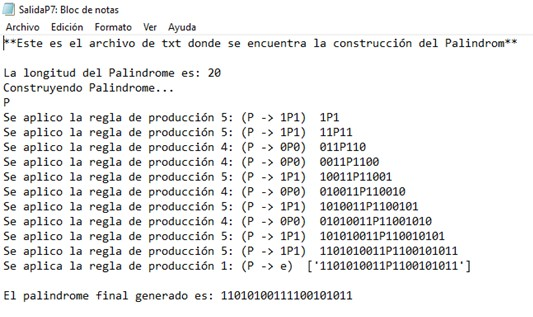
\includegraphics[height = 4cm]{MM2.jpg}
		\end{itemize}				
		\item \textbf{Modo Automático}
		\begin{itemize}
			\item 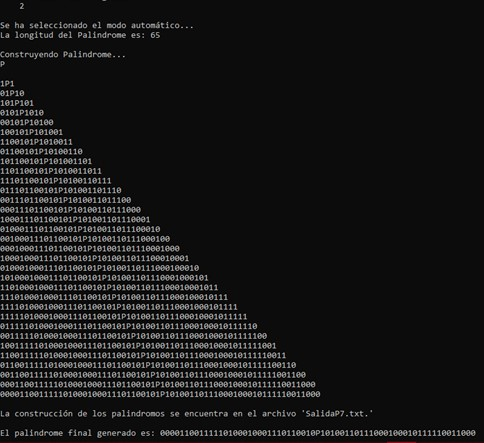
\includegraphics[height = 4cm]{MA1.jpg}
			\item 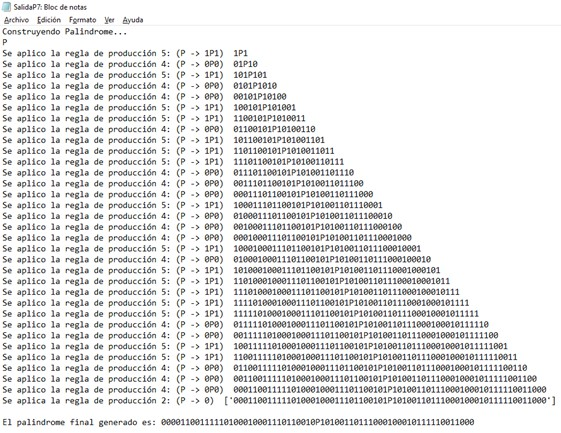
\includegraphics[height = 4cm]{MA2.jpg}
		\end{itemize}
	\end{enumerate}
	\section*{Código}
	\begin{python}
		# Programa 7.Palindromes
		# Nombre: Colín Ramiro Joel
		# Profesor: Juarez Martínez Genaro
		# Grupo: 4CM2
		# Materia: Teoría Computacional
		
		from random import randint
		
		def palindrome(opcion):
			archivo = open("SalidaP7.txt","w")
			archivo.write("**Este es el archivo de txt donde se encuentra la construcción del Palindrome**\n\n")
			if opcion == 1:
				print("\nSe ha seleccionado el modo manual...")
				longPalindrome = int(input("Digite la longitud: "))
			elif opcion == 2:
				print("\nSe ha seleccionado el modo automático...")
				longPalindrome = randint(1,100000)
			print("La longitud del Palindrome es: " + str(longPalindrome) + "\n")
			archivo.write("La longitud del Palindrome es: " + str(longPalindrome) + "\n")
			longPal2 = int(longPalindrome / 2)
			if(longPalindrome % 2) != 0:
				impar = True		        
			else:
				impar = False
			palindrome = "P"
			print("Construyendo Palindrome...\n" + palindrome + "\n")
			archivo.write("Construyendo Palindrome...\n" + palindrome + "\n")			
			for i in range(0, longPal2 + 1):
				if (i == longPal2):
					finPalin = palindrome.split()
					if(impar == False): #Regla de Producción (1) P -> e
						archivo.write("Se aplica la regla de producción 1: (P -> e)  ")
						archivo.write(str(finPalin) + "\n")
					if(impar == True): 
						regla_2_3 = randint(2,3)            
						if(regla_2_3 == 2): #Regla de Producción (2) P -> 0
							archivo.write("Se aplica la regla de producción 2: (P -> 0)  ")
							palindrome = "0" + palindrome                    
							print(palindrome)
							archivo.write(str(finPalin) + "\n")    			
						if(regla_2_3 == 3): #Regla de Producción (3) P -> 1
							archivo.write("Se aplico la regla de producción 3: (P -> 1)  ")
							palindrome =  "1" + palindrome
							print(palindrome)
							archivo.write(str(finPalin) + "\n")
				else:
					regla_4_5 = randint(4,5)
					if (regla_4_5 == 4): #Regla de Producción (4) P -> 0P0
						archivo.write("Se aplico la regla de producción 4: (P -> 0P0)  ")
						palindrome = "0" + palindrome + "0"
						print(palindrome)						
						archivo.write(str(palindrome) + "\n")
					if (regla_4_5 == 5): #Regla de Producción (5) P -> 1P1
						archivo.write("Se aplico la regla de producción 5: (P -> 1P1)  ")
						palindrome = "1" + palindrome + "1"
						print(palindrome)
						archivo.write(str(palindrome) + "\n")
			      
			print("\nLa construcción de los palindromos se encuentra en el archivo 'SalidaP7.txt.'")
			print("\nEl palindrome final generado es: " + palindrome[0:longPal2] + palindrome[longPal2+1::]+ "\n")  
			archivo.write("\nEl palindrome final generado es: " + palindrome[0:longPal2] + palindrome[longPal2+1  ::]+ "\n")         
		
		opc = 0
		salir = 3
		while opc != salir:
			print("***Menú Principal Programa 7***")    
			print("¿Cómo será la longitud?")
			opc = int(input('''
			1.- Longitud Manual
			2.- Longitud Aleatoria
			3.- Salir del Programa    
			'''))   
			if (opc == 1) or (opc == 2):
				palindrome(opc)    
			elif opc == 3:
				print("Saliendo del Programa. Hasta Luego!!!!")    
			else:
				print("Opción inválida, Vuelva a intentar")		
	\end{python}

	\section*{Conclusiones}
	En esta sección se encuentran las conclusiones de la práctica.
	Me apoye de las láminas presentadas en clase, asi como de otros recursos encontrados en diferentes páginas web relacionadas con el tema, para la realización del programa asi como para reforzar los conocimientos esperados. 
	En cuanto al programa puedo concluir que a mi parecer fue el más sencillo de implementar en comparación de los otros, ya que como también se puede observar en el código, es el más pequeño por asi decirlo en cuanto a líneas de código y también en cuanto al tiempo efectivo de realización.
	
	\section*{Referencias}
	\begin{enumerate}
		\item J. Andres Montoya. (2016). Introduccion a la teoria de la computacion: via palindromos. Diciembre 21, 2021, de Universidad Industrial de Santander Sitio web: http://matematicas.uis.edu.co/jmontoya/sites/default/files/algoritmos-automatas-tiempo-real.pdf
		\item Terry Anderson, Narad Rampersad, Nicolae Santean, and Jeffrey Shallit. (2019). Finite Automata, Palindromes, Powers, and Patterns. Diciembre 21,2021, de University of Waterloo Sitio web: https://cs.smu.ca/~nic.santean/art/pal.pdf
		\item Línea de Código. (2007). Palíndromos con Java. Diciembre 21,2021, de Línea de Código Sitio web: https://lineadecodigo.com/java/saber-si-una-palabra-es-un-palindromo-con-java/
		
	\end{enumerate}
	

	
\end{document}